\documentclass{article}

\usepackage{geometry}
\usepackage{amsmath}
\usepackage{graphicx}
\usepackage{listings}
\usepackage{hyperref}
\usepackage{multicol}
\usepackage{fancyhdr}
\pagestyle{fancy}
\hypersetup{ colorlinks=true, linkcolor=black, filecolor=magenta, urlcolor=cyan}
\geometry{ a4paper, total={170mm,257mm}, top=20mm, right=20mm, bottom=20mm, left=20mm}
\setlength{\parindent}{0pt}
\setlength{\parskip}{1em}
\renewcommand{\headrulewidth}{0pt}
\lhead{Competitive Programming - Arkavidia VI}
\fancyfoot[CE,CO]{\thepage}
\lstset{
    basicstyle=\ttfamily\small,
    columns=fixed,
    extendedchars=true,
    breaklines=true,
    tabsize=2,
    prebreak=\raisebox{0ex}[0ex][0ex]{\ensuremath{\hookleftarrow}},
    frame=none,
    showtabs=false,
    showspaces=false,
    showstringspaces=false,
    prebreak={},
    keywordstyle=\color[rgb]{0.627,0.126,0.941},
    commentstyle=\color[rgb]{0.133,0.545,0.133},
    stringstyle=\color[rgb]{01,0,0},
    captionpos=t,
    escapeinside={(\%}{\%)}
}

\begin{document}

\begin{center}
    \section*{Tantangan Penjaga Pintu} % ganti judul soal

    \begin{tabular}{ | c c | }
        \hline
        Batas Waktu  & 1s \\    % jangan lupa ganti time limit
        Batas Memori & 64MB \\  % jangan lupa ganti memory limit
        \hline
    \end{tabular}
\end{center}

\subsection*{Deskripsi}

Elza, seorang pendekar pengembara, mengabdikan hidupnya untuk menumpas kejahatan dan membantu yang lemah. Dalam pengembaraannya melewati suatu desa, dia melihat seorang anak kecil menangis terisak-isak. Elza pun menanyakan kepada anak itu kenapa dia menangis. Ternyata, anak itu hari ini sedang berulang tahun, tetapi dia tidak mempunyai pisau untuk memotong dan membagikan kue ulang tahunnya kepada teman-temannya. Elza lalu mengeluarkan pedang kepercayaannya yang tentunya sangat higienis untuk memotong kue pesta anak tersebut menjadi beberapa bagian.

Kue pesta memiliki bentuk segi-N beraturan. Elza si pendekar handal ingin hanya menggunakan satu gerakan untuk membagi kue tersebut. Pertama, Elza meletakkan ujung pedangnya di titik sudut kue terdekat dengan dirinya, lalu Elza mulai menggerakan ujung pedangnya ke titik sudut lain sehingga

\begin{itemize}
    \setlength\itemsep{0pt}
    \item Titik yang hendak dituju tidak bersebelahan dengan posisi sekarang
    \item Garis potongan yang hendak dibentuk tidak boleh berhimpitan atau berpotongan dengan garis potongan sebelumnya kecuali di titik sudut kue
\end{itemize}

Elza terus menggerakan pedangnya seperti ini sampai tidak ada gerakan valid yang dapat dilakukan. Saat Elza sedang sibuk memotong kue tersebut, anak kecil itu penasaran berapa banyak kah kemungkinan potongan yang dapat terjadi dengan aturan pemotongan seperti ini. Bantulah anak kecil ini menyelesaikan permasalahan tersebut untuk membuat hari ulang tahun terbaik untuknya. Perhatikan bahwa karena jawabannya mungkin sangat besar, cukup keluarkan jawabannya $\mod 10^9 + 7$.

\subsection*{Format Masukan}
Baris pertama terdiri dari satu bilangan bulat positif $N$ ($4 \leq N \leq 10^{18}$), menyatakan banyaknya titik sudut kue.

\subsection*{Format Keluaran}
Sebuah baris yang menyatakan banyaknya cara pemotongan yang ada, $\mod 10^9 + 7$.
\\

\begin{multicols}{2}
\subsection*{Contoh Keluaran}
\begin{lstlisting}
5
\end{lstlisting}
\begin{lstlisting}
6
\end{lstlisting}
\columnbreak
\subsection*{Contoh Keluaran}
\begin{lstlisting}
2
\end{lstlisting}
\begin{lstlisting}
6
\end{lstlisting}
\end{multicols}

\subsection*{Penjelasan}
Untuk segienam, ada enam kemungkinan potongan.

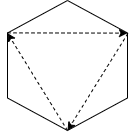
\includegraphics[width=40px]{1.png}
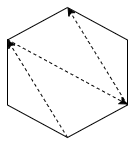
\includegraphics[width=40px]{2.png}
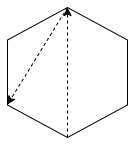
\includegraphics[width=40px]{3.png}
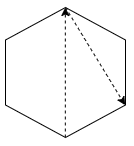
\includegraphics[width=40px]{4.png}
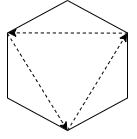
\includegraphics[width=40px]{5.png}
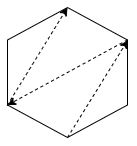
\includegraphics[width=40px]{6.png}


\pagebreak

\end{document}

